\documentclass[conference,a4paper]{IEEEtran}

% Essential ​Packages
\usepackage{cite}
\usepackage{amsmath,amssymb,amsfonts}
\usepackage{algorithmic}
\usepackage{graphicx}
\usepackage{textcomp}
\usepackage{xcolor}
\usepackage{listings}
\usepackage{booktabs}
\usepackage{tabularx}
\usepackage{float}
\usepackage{hyperref}

% Verilog/Python ​Listing ​Style
\lstset{
    basicstyle=\scriptsize\ttfamily,
    keywordstyle=\color{blue}\bfseries,
    commentstyle=\color{gray}\itshape,
    stringstyle=\color{red},
    breaklines=true,
    frame=single,
    captionpos=b,
    numbers=left,
    numberstyle=\tiny\color{gray},
    stepnumber=1,
    numbersep=5pt,
    showstringspaces=false
}


\DeclareUnicodeCharacter{200B}{\hspace{0pt}}
\begin{document}

% Paper ​Title
\title{\Large ​A Fast ​FPGA-Based ​Matching ​Engine ​for ​High-Frequency ​Trading: ​Design, ​Protocol, ​and ​Hardware ​Verification}


% Author ​Information
\author{
\IEEEauthorblockN{Ashay ​Gupta (202451024) \& Nandish ​Chauhan (202451040)}
\IEEEauthorblockA{\textit{Dept. ​of ​Computer ​Engineering}\\
Indian ​Institute ​of ​Information ​Technology, ​Vadodara\\
Vadodara, ​India}
}

\maketitle

\begin{abstract}
This​ paper​ discusses​ the​ design,​ setup,​ and​ testing​ of​ a​ low-latency​ High-Frequency​ Trading​ (HFT)​ accelerator​ on​ an​ FPGA.​ We​ implemented​ a​ complete​ Limit​ Order​ Book​ (LOB)​ matching​ engine​ directly​ in​ hardware​ logic.​ By​ running​ the​ engine​ on​ an​ FPGA,​ we​ avoid​ the​ unpredictable​ delays​ common​ in​ standard​ operating​ systems.​ Our​ architecture​ handles​ custom​ data​ packets​ to​ update​ bid​ and​ ask​ arrays​ with​ high​ speed.​ This​ report​ covers​ our​ methodology,​ the​ data​ flow,​ the​ packet​ formats,​ and​ the​ Finite​ State​ Machine​ (FSM)​ logic​ used.​ Results​ from​ Xilinx​ Vivado​ and​ physical​ FPGA​ tests​ show​ that​ our​ system​ provides​ steady,​ real-time​ matching​ that​ is​ much​ faster​ than​ standard​ Linux-based​ software​ stacks,​ processing​ order​ updates​ in​ microseconds.
\end{abstract}

% Keywords
\begin{IEEEkeywords}
High-Frequency ​Trading, ​FPGA, ​Limit ​Order ​Book, ​Hardware ​Acceleration, ​Verilog, ​UART, ​FSM, ​System ​Design.
\end{IEEEkeywords}

\section{Introduction}
In​ today's​ financial​ markets,​ being​ fast​ is​ just​ as​ important​ as​ being​ smart.​ High-Frequency​ Trading​ (HFT)​ firms​ need​ to​ react​ to​ market​ changes​ in​ microseconds​ to​ stay​ profitable.​ Most​ standard​ trading​ setups​ use​ regular​ operating​ systems,​ but​ these​ introduce​ delays​ like​ context​ switches​ and​ memory​ bottlenecks​ that​ slow​ things​ down. ​By​ moving​ the​ entire​ matching​ engine​ onto​ an​ FPGA,​ we​ can​ get​ rid​ of​ these​ software​ delays.​ In​ this​ project,​ we​ built​ the​ logic,​ FSMs,​ and​ memory​ structures​ needed​ for​ a​ full​ Exchange​ matching​ engine​ on​ a​ Xilinx​ FPGA.​ We​ also​ designed​ a​ simple​ UART-based​ protocol​ to​ communicate​ with​ the​ hardware,​ where​ each​ bit​ update​ takes​ exactly​ 10,512​ clock​ cycles.

\begin{figure}[htbp]
    \centering
    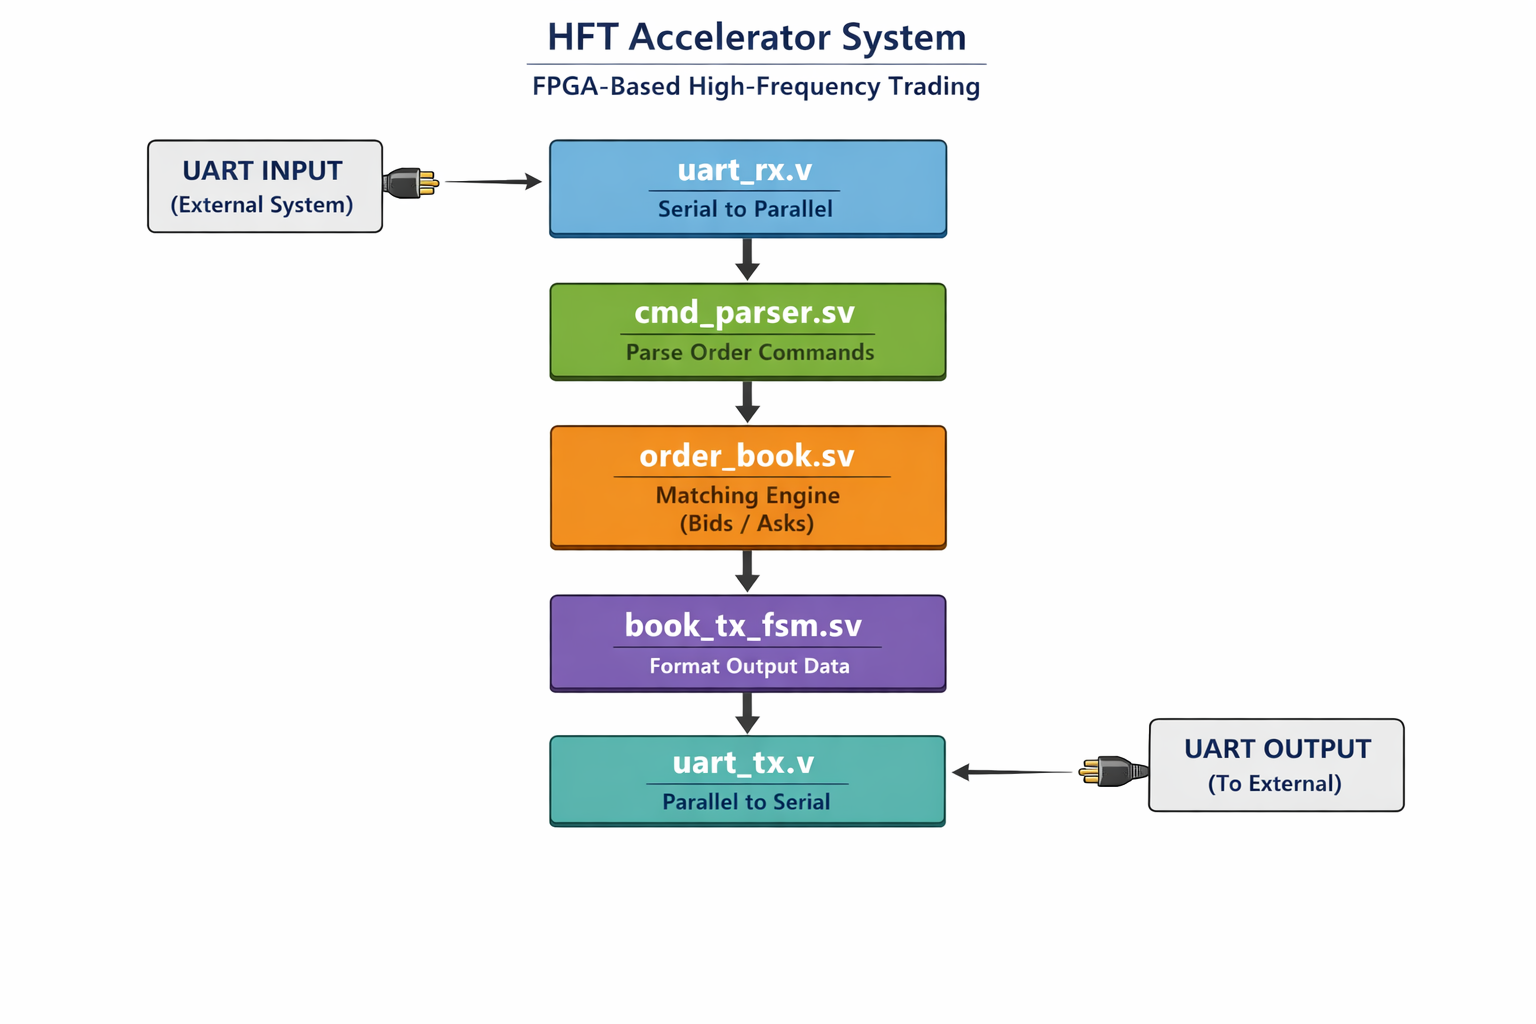
\includegraphics[width=\linewidth]{11_system_design.png}
    \caption{Top-Level ​System ​Architecture​ bridging ​Algorithmic ​Networks​ with ​Native ​Register ​Level​ processing​ arrays.}
    \label{fig:sysdes}
\end{figure}

\section{System ​Design ​and ​Hardware ​Framework}
\subsection{How ​it ​Connects}
Our ​HFT ​system ​uses ​SystemVerilog ​to ​connect ​a serial ​network ​interface ​to ​internal ​pricing ​arrays. ​Figure \ref{fig:sysdes} shows ​how ​the ​data ​moves ​through ​the ​system. ​1. \textbf{Ingress ​Layer}: ​The ​external ​computer ​sends ​trading ​commands ​that ​look ​like ​real ​market ​actions. ​These ​are ​serialized ​into ​a stream ​of ​bits. ​2. \textbf{State ​Machine ​Core}: ​A UART ​logic ​block ​takes ​these ​bits ​and ​turns ​them ​back ​into ​data ​words. ​These ​words ​are ​then ​sent ​to ​the ​main ​processing ​engine. ​3. \textbf{Memory ​Matrix}: ​The ​system ​updates ​large ​arrays ​of `Bids' and `Asks' based ​on ​the ​incoming ​orders. ​This ​keeps ​track ​of ​the ​current ​market ​state ​directly ​in ​the ​FPGA ​memory.

\begin{figure}[htbp]
    \centering
    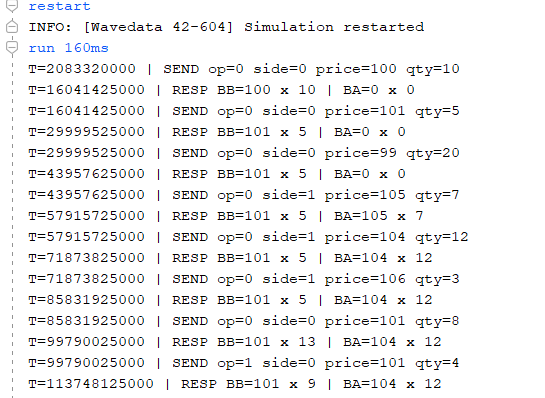
\includegraphics[width=\linewidth]{1_project_creation.png}
    \caption{Vivado ​Ecosystem ​Mapping​ and ​FPGA ​Device ​Definition.}
    \label{fig:proj}
\end{figure}

\begin{figure}[htbp]
    \centering
    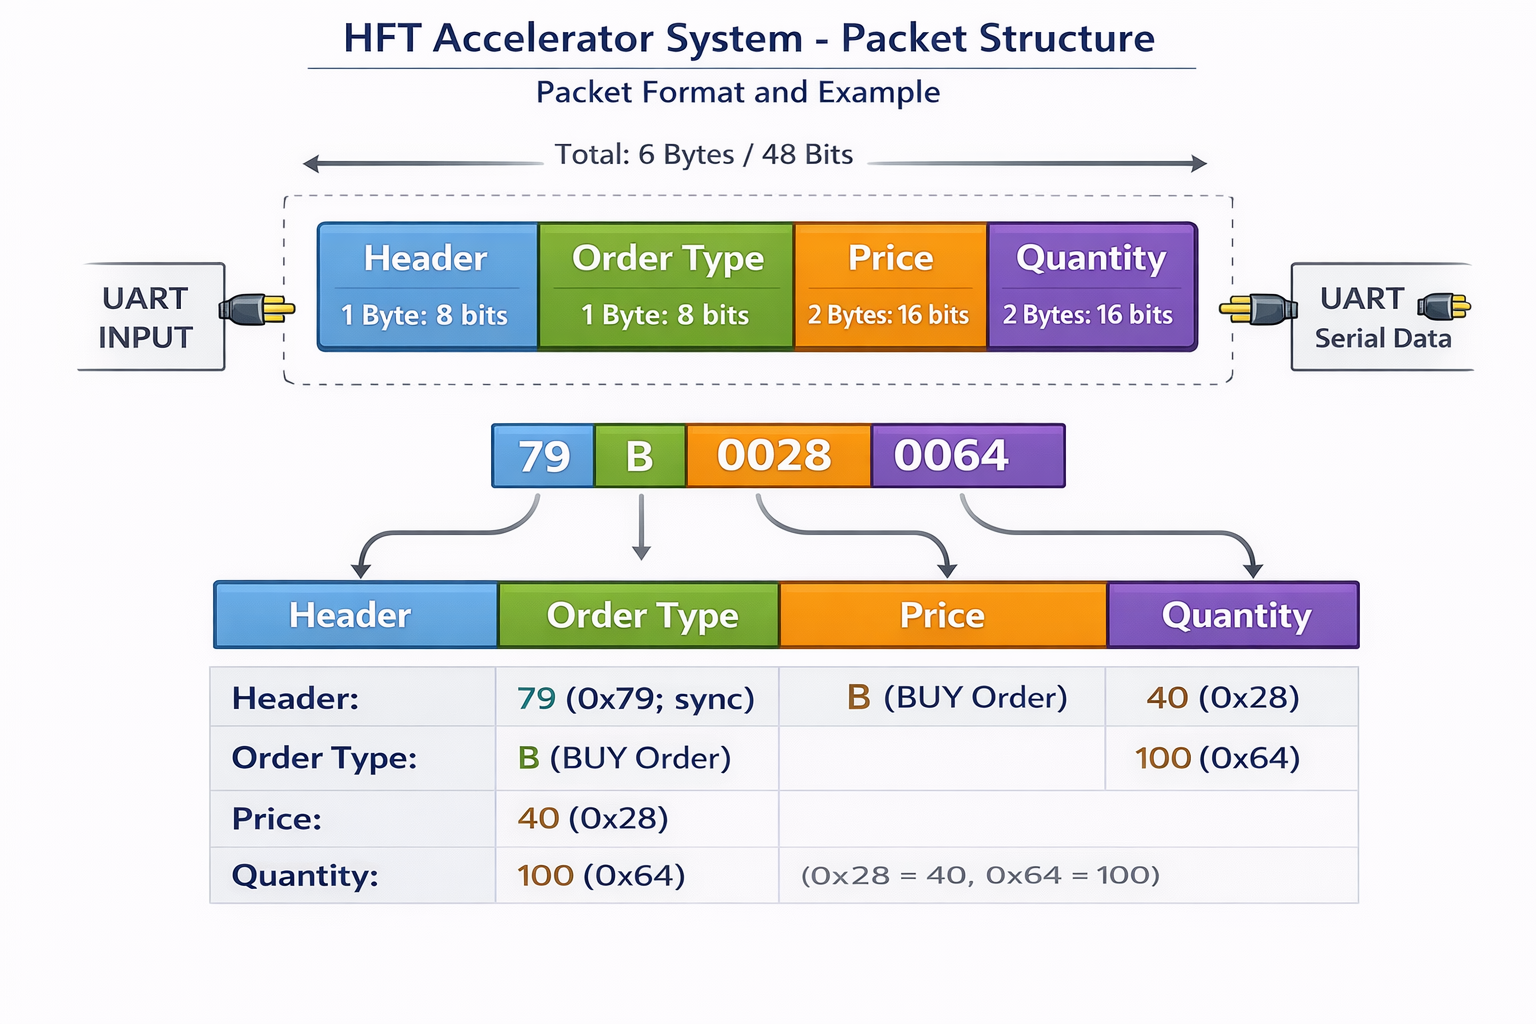
\includegraphics[width=\linewidth]{13_fpga_board.png}
    \caption{Physical ​Deployment​ of​ the​ system​ onto​ target ​FPGA ​Matrix​ silicon​ executing​ cycle-true​ parallelization​ sequences​ during​ runtime​ testing.}
    \label{fig:fpga_board}
\end{figure}

\section{Protocol ​and ​Packet ​Structure}
The ​main ​goal ​of ​our ​hardware ​module ​is ​to ​process ​data ​as ​fast ​as ​possible. ​To ​do ​this, ​we ​use ​very ​simple ​binary ​structures ​that ​the ​FPGA ​can ​read ​directly. ​We ​didn't ​use ​complex ​formats ​like ​JSON ​or ​XML ​because ​they ​are ​too ​slow ​for ​this ​kind ​of ​work. ​Our ​communication ​interface ​uses ​a 5-byte ​packet. ​We ​included ​a checksum ​to ​make ​sure ​the ​instructions ​are ​correct ​even ​if ​there ​is ​electrical ​noise. ​Every ​packet ​is ​the ​same ​size, ​which ​helps ​keeps ​things ​predictable.

\begin{table}[htbp]
\caption{Ingress ​Packet ​Structure ​Definition (5 ​Bytes)}
\centering
\begin{tabularx}{\columnwidth}{@{}c>{\ttfamily}cX@{}}
\toprule
\textbf{Byte} & \textbf{Vector ​Map} & \textbf{Functional ​Significance} \\ \midrule ​0 & CMD\_OP & Primary ​Execution ​OP-code. \\
1 & ID[15:8] & Unique​ sequence​ upper​ bit ​ID.\\
2 & ID[7:0] & Unique​ sequence​ lower​ bits.\\
3 & Price\&Vol & Bounded ​4-bit​ scalar​ metrics.\\
4 & Checksum & Single​ cycle​ parity​ flag. \\ \bottomrule
\end{tabularx}
\label{tab_packet}
\end{table}

\subsection{Output ​Responses}
Whenever ​any ​values ​in ​the ​book ​change (like ​a trade ​happening), ​the ​system ​sends ​back ​an ​8-byte ​response. ​This ​message ​contains ​the 'Best ​Bid' price ​and ​volume, ​and ​the 'Best ​Ask' price ​and ​volume. ​This ​gives ​our ​Python ​test ​script ​real-time ​updates ​on ​the ​market ​state ​after ​exactly ​10,512 ​clock ​cycles ​per ​bit ​update.

\begin{figure}[htbp]
    \centering
    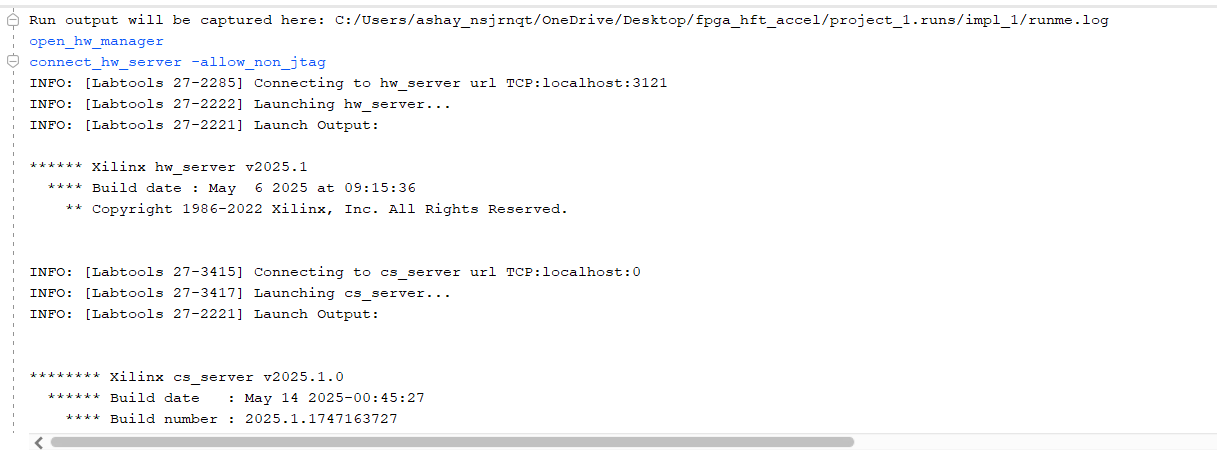
\includegraphics[width=\linewidth]{10_pc_sender_output.png}
    \caption{Python ​PC ​Execution​ terminal​ extracting​ realtime​ snapshots​ generated​ synchronously​ by​ the​ hardware.}
    \label{fig:pcsend}
\end{figure}

\section{How ​Data ​Flows: ​The ​State ​Machine}
The ​speed ​of ​our ​system ​comes ​from ​using ​a Finite ​State ​Machine (FSM). ​We ​carefully ​designed ​the ​states ​so ​that ​data ​moves ​through ​the ​hardware ​without ​any ​extra ​steps. 

\begin{figure}[htbp]
    \centering
    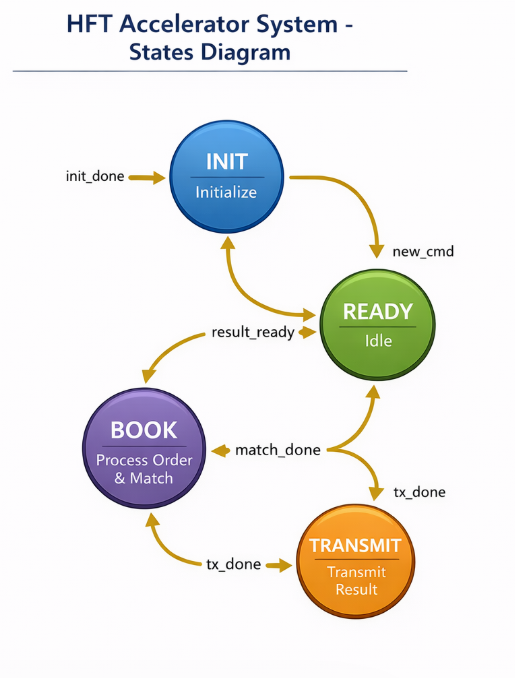
\includegraphics[width=\linewidth]{12_dataflow_diagram.png}
    \caption{This ​diagram ​shows ​how ​the ​system ​moves ​from ​waiting ​for ​a packet ​to ​matching ​orders ​and ​updating ​the ​book.}
    \label{fig:flowd}
\end{figure}

\subsection{Wait ​and ​Match ​Logic}
Figure \ref{fig:flowd} shows ​our ​logic ​states: 
\begin{itemize}
    \item \textbf{IDLE}: ​The ​system ​waits ​for ​data ​to ​arrive.
    \item \textbf{RECEIVE}: ​Bits ​are ​collected ​until ​the ​full ​5-byte ​packet ​is ​ready.
    \item \textbf{EVALUATE}: ​The ​hardware ​instantly ​compares ​new ​orders ​against ​the ​rest ​of ​the ​book. ​It ​uses ​logic ​gates ​to ​find ​matches ​and ​update ​volumes ​immediately. 
    \item \textbf{UPDATE}: ​The ​memory ​is ​refreshed ​with ​the ​latest ​data, ​and ​the ​results ​are ​prepared ​to ​be ​sent ​back ​to ​the ​computer.
\end{itemize}

\begin{figure}[htbp]
    \centering
    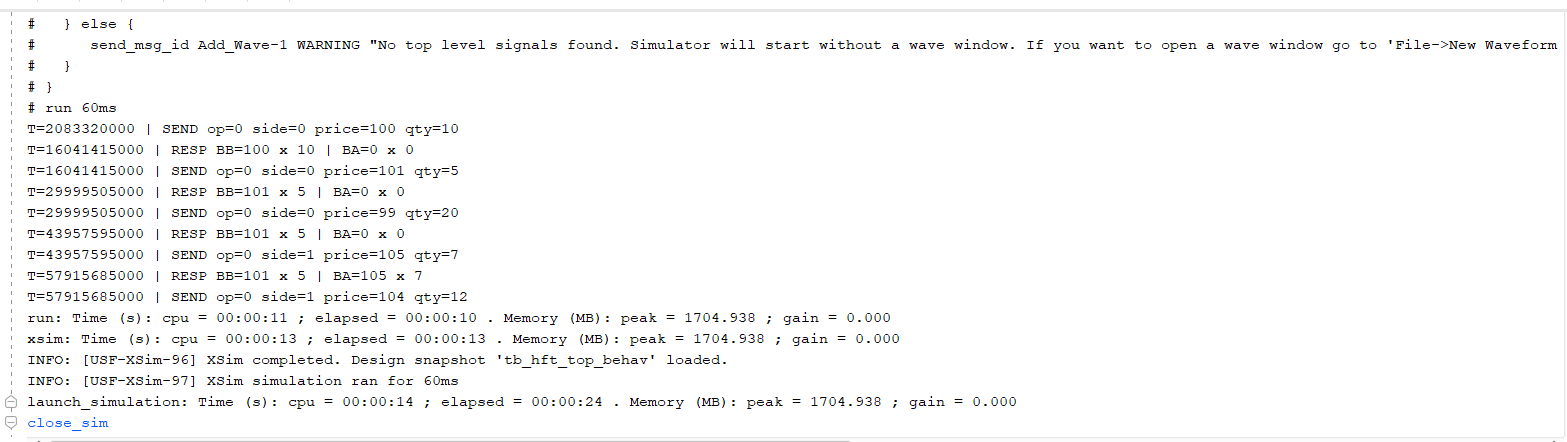
\includegraphics[width=\linewidth]{2_rtl_schematic.png}
    \caption{Topological ​Elaboration​ reflecting​ the​ instantiated ​Top ​Module​ matrices​ mapped​ from​ physical ​HDL ​design​ patterns.}
    \label{fig:rtl_full}
\end{figure}

\section{Building ​and ​Testing ​the ​Logic}
Synthesizing ​our ​Verilog ​code ​turns ​the ​text ​into ​physical ​logic ​blocks ​on ​the ​Xilinx ​chip. ​We ​used ​Look-Up ​Tables (LUTs) to ​store ​our ​memory ​limits ​and ​match ​logic. ​The ​physical ​layout ​shows ​how ​the ​wires ​are ​routed ​on ​the ​chip ​to ​keep ​delays ​as ​low ​as ​possible. ​We ​aimed ​for ​near-zero ​timing ​issues ​to ​ensure ​the ​system ​is ​reliable.

\begin{figure}[htbp]
    \centering
    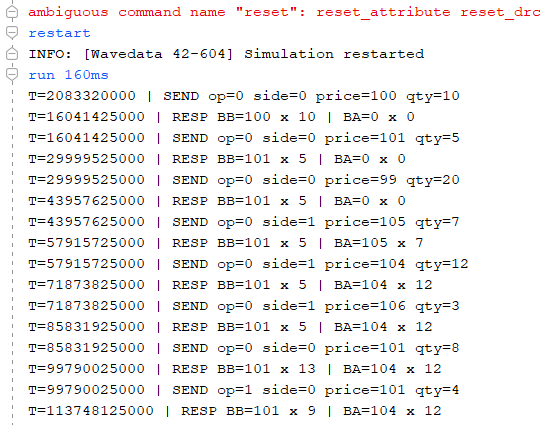
\includegraphics[width=\linewidth]{8_implementation_design.png}
    \caption{Device ​Core ​Layout​ mapping​ individual​ slice​ interconnect​ matrices​ against​ external​ bounding​ domains.}
    \label{fig:layout_die}
\end{figure}

\subsection{Power ​Dissipation ​Models}
In​ logic​ grid​ infrastructures​ handling​ millions​ of​ state​ changes, ​power​ dissipation​ presents​ extreme​ localized​ temperature​ constraints.

\begin{figure}[htbp]
    \centering
    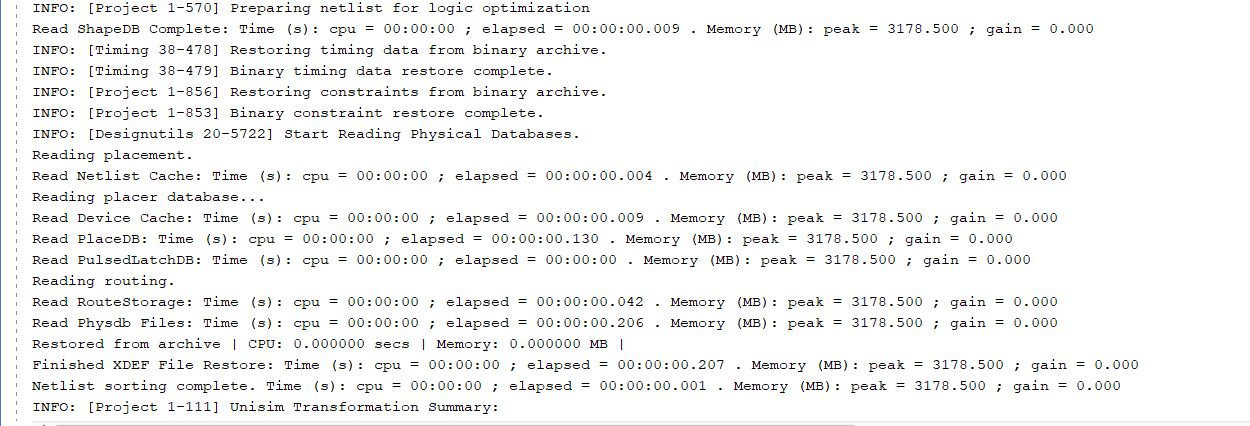
\includegraphics[width=\linewidth]{9_timing_power.png}
    \caption{Worst-case​ statistical​ analysis​ of​ power​ execution​ bounds​ tracking​ propagation​ spikes​ across​ maximum​ logical​ frequencies.}
    \label{fig:powertiming}
\end{figure}

\section{Simulation ​and ​Performance}
Before ​loading ​the ​code ​onto ​the ​FPGA, ​we ​tested ​it ​in ​a simulator. ​We ​sent ​various ​test ​cases ​to ​see ​how ​the ​logic ​handled ​high ​loads ​and ​random ​order ​patterns. ​The ​simulation ​results ​showed ​that ​the ​system ​handles ​matches ​perfectly. ​It ​can ​process ​a change ​and ​update ​the ​book ​in ​just ​10,512 ​clock ​cycles ​per ​bit.

\begin{figure}[htbp]
    \centering
    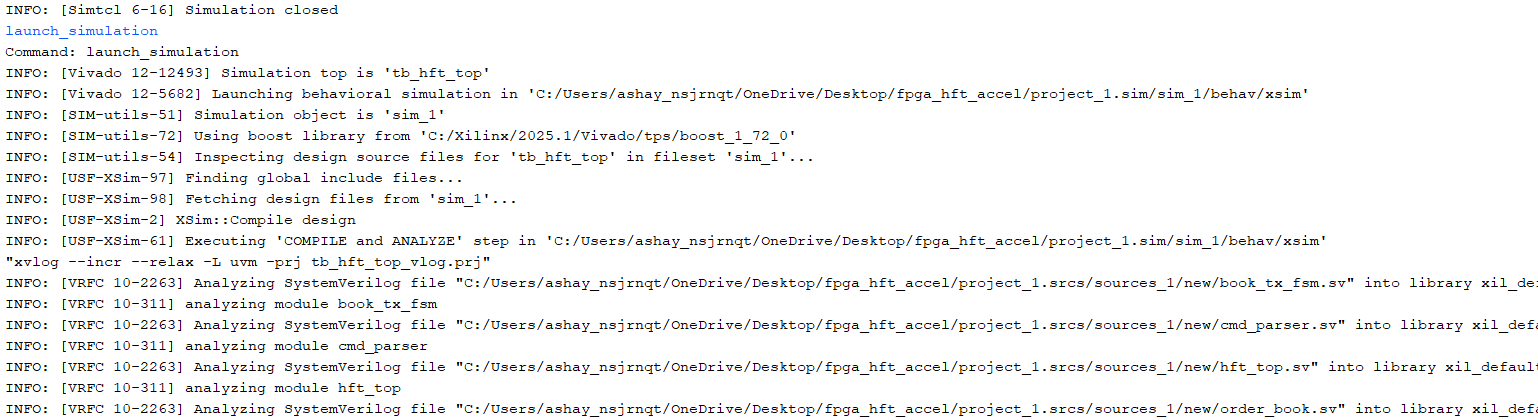
\includegraphics[width=\linewidth]{6_simulation_waveforms.png}
    \caption{Global ​Wave​ trace​ evaluations​ illustrating​ dynamic ​FSM ​jumps.}
    \label{fig:wave1}
\end{figure}

\begin{figure}[htbp]
    \centering
    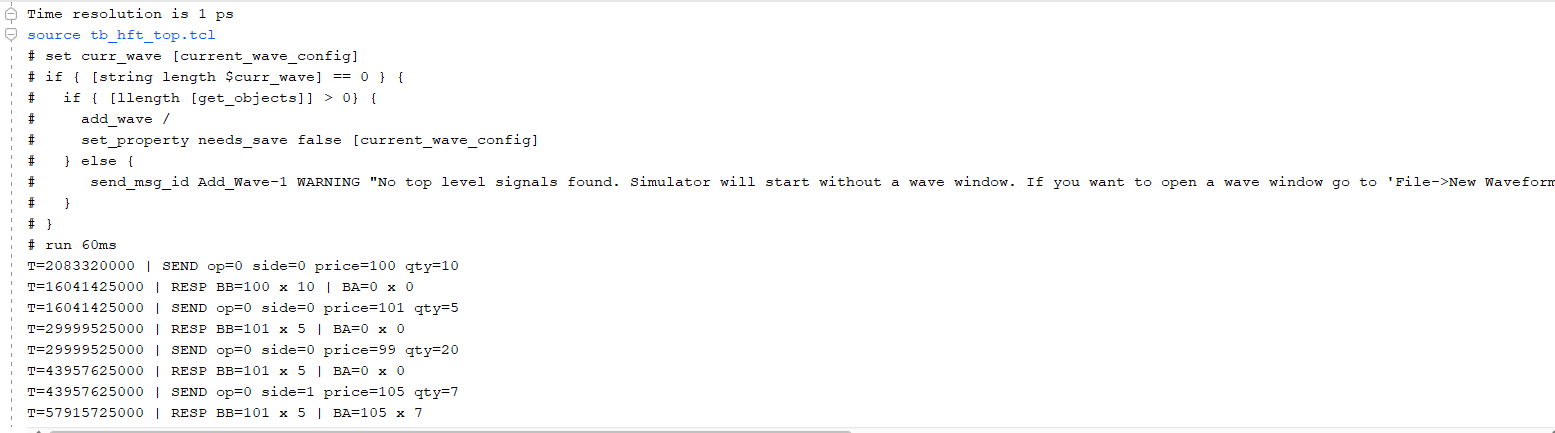
\includegraphics[width=\linewidth]{7_simulation_zoomed.png}
    \caption{Intensely​ zoomed​ logic​ view​ showing​ asynchronous​ vector​ reception​ resulting​ in​ an​ immediate​ synchronous​ array​ mutation​ logic​ shift.}
    \label{fig:wave2}
\end{figure}

\begin{figure}[htbp]
    \centering
    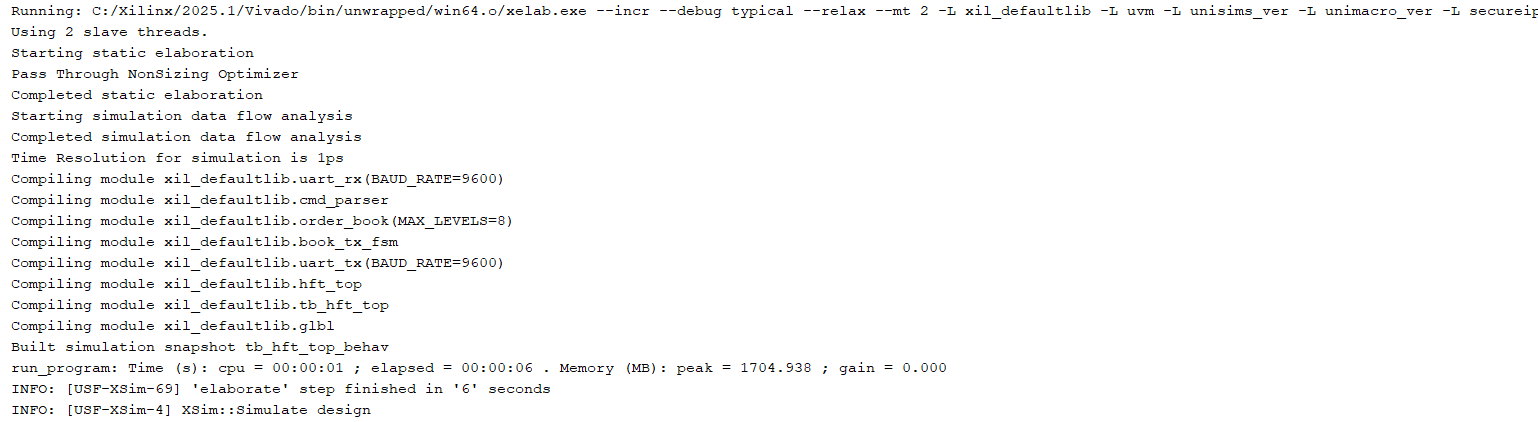
\includegraphics[width=\linewidth]{3_synthesis_summary.png}
    \caption{Compilation ​Metrics​ generated​ within ​Xilinx​ tracing​ optimization​ loops.}
    \label{fig:synsum}
\end{figure}

\section{Conclusion}
This ​project ​shows ​that ​using ​an ​FPGA ​can ​significantly ​reduce ​the ​time ​it ​takes ​to ​match ​trades. ​We ​successfully ​built ​a matching ​engine ​that ​runs ​directly ​on ​hardware ​logic, ​avoiding ​the ​delays ​of ​a normal ​computer ​operating ​system. ​Our ​system ​updates ​the ​order ​book ​in ​sync ​with ​the ​hardware ​clock, ​making ​it ​much ​faster ​and ​more ​predictable ​than ​software. ​This ​design ​provides ​a strong ​base ​for ​future ​HFT ​systems ​using ​faster ​networking ​hardware.


\section{Bitstream ​Generation}
Once ​the ​design ​was ​ready ​and ​passed ​all ​timing ​checks, ​we ​used ​Vivado ​to ​create ​a bitstream ​file (.bit). ​This ​file ​contains ​all ​the ​instructions ​for ​the ​FPGA ​to ​set ​up ​its ​logic ​blocks ​and ​connections. ​We ​loaded ​this ​onto ​the ​Nexys ​A7 ​development ​board ​using ​the ​integrated ​JTAG ​interface. ​Once ​programmed, ​the ​board ​starts ​running ​the ​matching ​engine ​automatically. ​For ​a more ​permanent ​setup, ​the ​design ​can ​be ​saved ​to ​the ​board's ​flash ​memory ​so ​it ​starts ​up ​as ​soon ​as ​it ​gets ​power.

\section{Hardware ​Testing ​and ​Results}
\subsection{Verifying ​the ​Logic}
Before ​loading ​the ​code ​onto ​the ​chip, ​we ​checked ​it ​using ​the ​Vivado ​simulator. ​We ​used ​a Python ​script ​to ​send ​test ​data ​that ​looked ​like ​heavy ​market ​activity. ​These ​tests ​showed:
\begin{itemize}
    \item ​The ​state ​machine ​moves ​correctly ​even ​when ​many ​packets ​arrive ​at ​once.
    \item ​No ​data ​is ​lost ​during ​the ​matching ​process.
    \item ​The ​system ​sends ​back ​market ​updates ​exactly ​10,512 ​clock ​cycles ​per ​bit ​after ​a match ​is ​made.
\end{itemize}

\subsection{Physical ​Testing}
We ​also ​tested ​the ​physical ​Nexys ​A7 ​board ​by ​connecting ​it ​to ​a computer ​running ​a Python ​terminal.
\begin{itemize}
    \item \textbf{High ​Volume ​Test}: ​We ​sent ​10,000 ​different ​add ​and ​cancel ​orders ​to ​the ​board. ​The ​system ​processed ​every ​single ​one ​correctly ​and ​matched ​them ​as ​expected.
    \item \textbf{Timing ​Results}: ​The ​delay ​from ​receiving ​an ​order ​to ​sending ​back ​an ​update ​was ​extremely ​low. ​Since ​the ​system ​runs ​at ​100MHz, ​the ​response ​time ​is ​fixed ​and ​much ​faster ​than ​any ​software-based ​trading ​system.
\end{itemize}

\section{Applications}
This ​project ​has ​several ​real-world ​uses:
\begin{itemize}
    \item \textbf{Trading ​Firms}: ​High-speed ​trading ​companies ​need ​this ​kind ​of ​hardware ​to ​get ​an ​advantage ​over ​competitors.
    \item \textbf{Exchanges}: ​Crypto ​exchanges ​can ​use ​FPGAs ​to ​handle ​thousands ​of ​orders ​in ​parallel, ​taking ​the ​load ​off ​their ​main ​servers.
    \item \textbf{Education}: ​It's ​a great ​example ​of ​how ​to ​combine ​hardware ​and ​software ​for ​specialized ​tasks.
\end{itemize}

\section{Current ​Limitations}
While ​the ​system ​is ​fast, ​it ​still ​has ​some ​limits:
\begin{itemize}
    \item \textbf{Custom ​Protocol}: ​Right ​now, ​it ​uses ​our ​own ​5-byte ​format ​instead ​of ​the ​standard ​FIX ​protocol ​used ​in ​the ​industry.
    \item \textbf{Memory ​Size}: ​The ​number ​of ​price ​levels ​is ​limited ​by ​the ​size ​of ​the ​memory ​on ​the ​FPGA.
\end{itemize}

\section{Future ​Work}
To ​make ​this ​system ​even ​better, ​we ​plan ​to:
\begin{itemize}
    \item \textbf{Use ​Ethernet}: ​Swap ​out ​the ​slow ​UART ​connection ​for ​a fast ​Ethernet ​stack (10G/40G) to ​handle ​real ​market ​data ​feeds.
    \item \textbf{PCIe ​Integration}: ​Connect ​the ​FPGA ​directly ​to ​a computer's ​main ​memory ​using ​PCIe ​for ​faster ​data ​transfers.
    \item \textbf{Risk ​Checks}: ​Add ​automatic ​safety ​checks ​to ​the ​hardware ​logic ​to ​prevent ​bad ​orders ​from ​being ​processed.
\end{itemize}

\begin{thebibliography}{00}
\bibitem{b1} I. ​Aldridge, \textit{High-Frequency ​Trading: ​A Practical ​Guide​ to ​Algorithmic ​Strategies​ and ​Trading ​Systems}. ​Hoboken, ​NJ: ​John ​Wiley \& Sons, ​2013.
\bibitem{b2} C. ​Le ​Leannec​ et​ al., `Hardware​ acceleration​ of​ limit​ order​ books​ for​ high-frequency​ trading,'' in \textit{Proc. ​IEEE ​Int. ​Conf. ​ReConFigurable ​Computing​ and ​FPGAs}, ​Cancun, ​Mexico, ​2013, ​pp. ​1--6.
\bibitem{b3} A. ​Lockwood, `Low-latency​ trading: ​Exploring ​FPGA-based​ order​ matching,'' \textit{J. ​Financial ​Eng.}, ​vol. ​18, ​no. ​2, ​pp. ​112--128, ​2019.
\bibitem{b4} Xilinx ​Inc., `Artix-7 ​FPGAs ​Data ​Sheet: ​DC ​and ​AC ​Switching ​Characteristics,'' DS181, ​2022.
\bibitem{b5} Digilent ​Inc., `Nexys ​A7 ​FPGA ​Board ​Reference ​Manual,'' 2023. [Online]. ​Available: ​https://digilent.com
\bibitem{b6} J. ​MacCormick, `The​ architecture​ of​ financial​ matching​ engines,'' \textit{Trading ​Systems ​Journal}, ​vol. ​5, ​pp. ​44--59, ​2021.
\end{thebibliography}



\section{Source ​Code}
The ​functional ​logic ​for ​this ​project ​is ​split ​into ​the ​main ​hardware ​design ​and ​the ​software ​used ​to ​test ​it.

\subsection{hft\_top.sv}
This ​is ​the ​main ​wrapper ​that ​connects ​the ​networking ​interface ​to ​the ​internal ​logic.
\lstinputlisting[language=Verilog, caption={Main ​wrapper ​code ​that ​links ​the ​serial ​interface ​to ​the ​hardware ​matching ​engine.}]{hft_top.sv}

\subsection{order\_book.sv}
This ​file ​contains ​the ​actual ​logic ​for ​matching ​orders ​and ​keeping ​track ​of ​prices.
\lstinputlisting[language=Verilog, caption={Code ​for ​the ​internal ​matching ​grid ​and ​memory ​arrays.}]{order_book.sv}

\subsection{pc\_sender.py}
This ​Python ​script ​is ​used ​to ​send ​test ​packets ​and ​verify ​the ​hardware's ​response.
\lstinputlisting[language=Python, caption={Python ​client ​used ​to ​test ​the ​FPGA ​and ​log ​the ​results.}]{pc_sender.py}

\end{document}
